% figures/state_machine.tex
% Standalone — compile with:
%   xelatex -interaction=nonstopmode state_machine.tex
\documentclass[tikz, border=4pt]{standalone}

%% ---------- Packages ----------
\usepackage{fontspec}
\usepackage{xcolor}
\usepackage{amsfonts}   % \mathbb
\usepackage{tikz}
\usetikzlibrary{positioning, arrows.meta}

%% ---------- Document ----------
\begin{document}
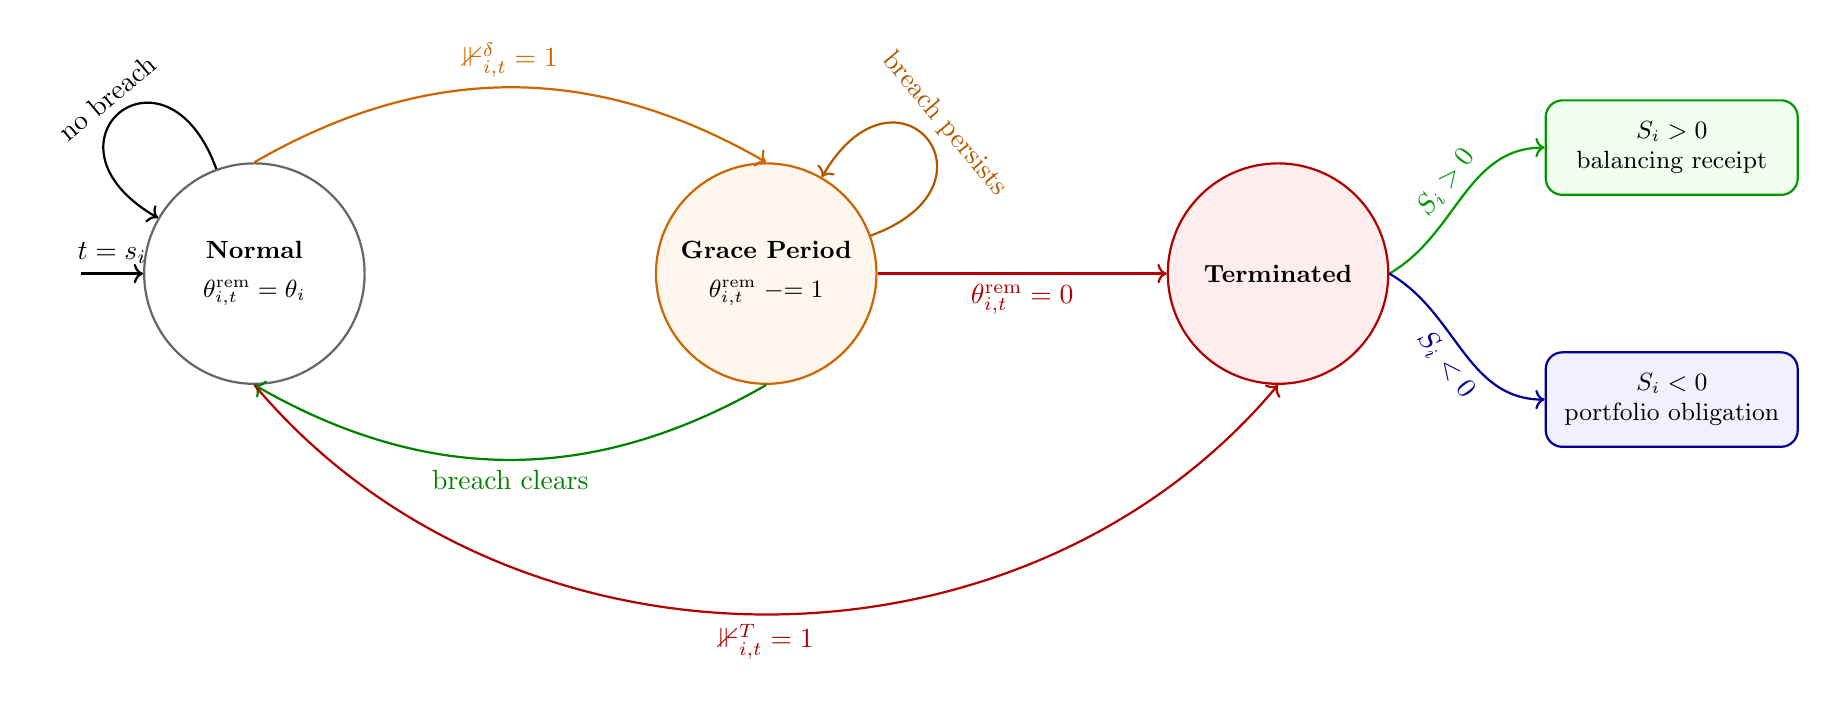
\begin{tikzpicture}[
    every node/.style={font=\small},
    state/.style={circle, draw=black!60, fill=white,
                  minimum size=2.8cm, align=center, thick},
    grace/.style={circle, draw=orange!80!black, fill=orange!7,
                  minimum size=2.8cm, align=center, thick},
    term/.style ={circle, draw=red!70!black,    fill=red!7,
                  minimum size=2.8cm, align=center, thick},
    posnode/.style={rectangle, rounded corners=6pt,
                    draw=green!60!black, fill=green!6,
                    minimum width=3.2cm, minimum height=1.2cm,
                    align=center, thick},
    negnode/.style={rectangle, rounded corners=6pt,
                    draw=blue!60!black, fill=blue!6,
                    minimum width=3.2cm, minimum height=1.2cm,
                    align=center, thick},
  ]

  % --- nodes ---
  \node[state] (normal) at (0,0)
    {\textbf{Normal}\\[3pt]
     $\theta^{\mathrm{rem}}_{i,t} = \theta_i$};

  \node[grace] (grace) at (6.5,0)
    {\textbf{Grace Period}\\[3pt]
     $\theta^{\mathrm{rem}}_{i,t} \mathrel{-}= 1$};

  \node[term] (term) at (13,0)
    {\textbf{Terminated}};

  \node[posnode] (posout) at (18, 1.6)
    {$S_i > 0$\\balancing receipt};

  \node[negnode] (negout) at (18,-1.6)
    {$S_i < 0$\\portfolio obligation};

  % --- entry arrow ---
  \draw[->, thick] (-2.2,0) -- (normal.west)
    node[midway, above, font=\normalsize] {$t = s_i$};

  % --- Normal self-loop: no breach ---
  \draw[->, thick, black]
    (normal) to[out=110, in=150, looseness=5]
    node[above, font=\normalsize, sloped] {no breach}
    (normal);

  % --- Normal -> Grace: Condition 1 fires ---
  \draw[->, thick, orange!80!black]
    (normal.north) to[out=30, in=150]
    node[above, font=\normalsize]
      {$\mathbb{1}^{\delta}_{i,t} = 1$}
    (grace.north);

  % --- Grace self-loop: breach persists ---
  \draw[->, thick, orange!70!black]
    (grace) to[out=20, in=60, looseness=5]
    node[above, font=\normalsize, sloped] {breach persists}
    (grace);

  % --- Grace -> Normal: breach clears ---
  \draw[->, thick, green!50!black]
    (grace.south) to[out=210, in=330]
    node[below, font=\normalsize] {breach clears}
    (normal.south);

  % --- Grace -> Terminated: counter exhausted ---
  \draw[->, thick, red!70!black]
    (grace.east) -- (term.west)
    node[midway, below, font=\normalsize]
      {$\theta^{\mathrm{rem}}_{i,t} = 0$};

  % --- Normal -> Terminated: Condition 2 fires (hard deadline) ---
  \draw[->, thick, red!70!black]
    (normal.south) to[out=-50, in=-130]
    node[below, font=\normalsize]
      {$\mathbb{1}^{T}_{i,t} = 1$}
    (term.south);

  % --- Terminated -> settlement outcomes ---
  \draw[->, thick, green!60!black]
    (term.east) to[out=30, in=180]
    node[midway, above, font=\normalsize, sloped] {$S_i > 0$}
    (posout.west);

  \draw[->, thick, blue!60!black]
    (term.east) to[out=-30, in=180]
    node[midway, below, font=\normalsize, sloped] {$S_i < 0$}
    (negout.west);

\end{tikzpicture}
\end{document}
